\scanpage{17}
whence at once the envisaged arrow.

It would still be necessary to make explicit how (7) (8) result from the datum of the action of $\unsure{\mathcal E|\Sigma}'$ on $\widetilde{\mathfrak X}'(J)$, inducing a \uline{free} action of $\pi_1\subset\unsure{\mathcal E|\Sigma}'$ on $\widetilde{\mathfrak X}'(J)$ (having $J$ as quotient set)\ldots.

\uline{Reformulation}

Consider the systems
\[
\left\{\begin{gathered}
\diagram{\begin{tikzcd}[ampersand replacement=\&]
1 \arrow[r,dash] \& \pi \arrow[r,dash] \& \unsure{\mathcal E|\Sigma} \arrow[r,dash] \& \mathcal G \arrow[r,dash] \& 1 \& \text{extension of groups}
\end{tikzcd}}\\
\mathfrak Z\quad\unsure{\mathcal E|\Sigma}\text{-set }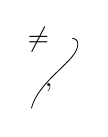
\begin{tikzpicture}[baseline=(comma.base)]
\node[anchor=base,inner sep=0pt] (comma) at (0,0) {$,$};
\node[anchor=base,inner sep=0pt] at (-.13,.50) {$\inserted{\ne\varnothing}$};
\draw[line width=.3pt] (-.22,-.28) .. controls (-.13,.06) and (.30,.29) .. (.36,.48) .. controls (.39,.58) and (.35,.60) .. (.30,.61);
\end{tikzpicture}\text{ where }\pi\subset\unsure{\mathcal E|\Sigma}\text{ acts freely}
\end{gathered}\right.
\]
They form a \uline{category} $C$

Consider the systems $(\Pi,\widetilde\Pi,p,\mathcal G,g)$ where $\Pi$ is a \begin{tikzpicture}[baseline=(word.base)]
\node[anchor=base west,inner sep=0pt] (word) at (0,0) {connected};
\node[anchor=base east,inner sep=0pt] at (.20,.52) {\inserted{\unsure{\begin{tikzpicture}[baseline=-.35ex,x=.5cm,y=.5cm,line cap=round]
\draw[line width=.35pt] (.07,.49) .. controls (.16,.46) and (.27,.39) .. (.27,.28)
  .. controls (.27,.13) and (.08,.11) .. (.09,.24)
  .. controls (.10,.34) and (.20,.39) .. (.25,.32);
\draw[line width=.45pt] (.46,.36)--(.68,.34);
\end{tikzpicture}}}};
\draw[line width=.3pt] (-.18,-.20) .. controls (-.28,.02) and (-.02,.27) .. (.36,.42) .. controls (.51,.50) and (.53,.57) .. (.40,.60);
\end{tikzpicture} groupoid, $p:\widetilde\Pi\longrightarrow\Pi$ a universal covering of $\Pi$, and $\mathcal G$ a group acting \deleted{\unsure{on|of}} on $\Pi$ by automorphisms via $a:\mathcal G\longrightarrow\operatorname{Aut}(\Pi)$. They form a category $C'$. We shall define equivalences quasi-inverse to one another
\diagram{\begin{tikzcd}[ampersand replacement=\&]
C \arrow[r,shift left,"\alpha"] \& C' \arrow[l,shift left,"\beta"]
\end{tikzcd}}
\mspage{16}
